\begin{figure}
	
	\begin{center}
		
		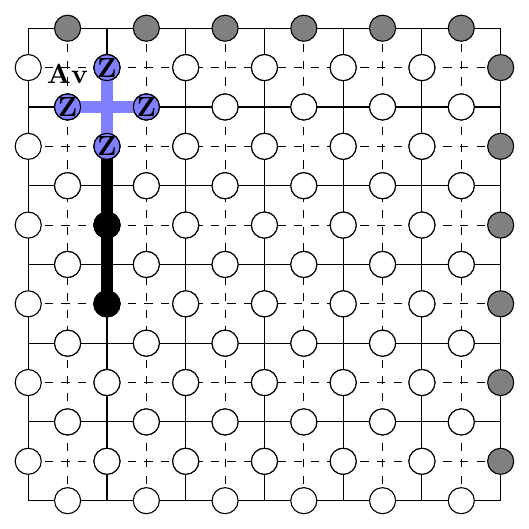
\begin{tikzpicture}
			% Draw dashed lines
			\foreach \i in {-3,-2.5,...,3}
			{
				\draw[dashed] (\i,-3) -- (\i,3);
			}
			\foreach \j in {-3,-2.5,...,3}
			{
				\draw[dashed] (-3,\j) -- (3,\j);
			}
			
			
			
			% Draw solid grid and nodes with circles in the middle of each side
			\draw[step=1cm] (-3,-3) grid (3,3);
			\foreach \i in {-2.5,...,2.5}
			{
				\foreach \j in {-2.5,...,2.5}
				{
					
					
					\begin{scope}[transform canvas={xshift=\i cm,yshift=\j cm}]
						\node[right,xshift=0.2cm,yshift=0.4cm] {};
						% Convert \j and \i to integers
						\pgfmathtruncatemacro{\intj}{\j}
						\pgfmathtruncatemacro{\inti}{\i}
						
						% Draw circles at the midpoints of each side
						\ifnum\intj=2
						\draw node[draw,circle,fill=gray] at (0,0.5) {};
						\else
						\draw node[draw,circle,fill=white] at (0,0.5) {};
						\fi
						
						\ifnum\inti=2
						\draw node[draw,circle,fill=gray] at (0.5,0) {};
						\else
						\draw node[draw,circle,fill=white] at (0.5,0) {};
						\fi
						
						\draw node[draw,circle,fill=white] at (0,-0.5) {};
						\draw node[draw,circle,fill=white] at (-0.5,0) {};
					\end{scope}
				}
			}
			
			\foreach \i in {-2,...,-2}
			{
				\draw[black, line width=1.5mm] (\i,-0.5) -- (\i,1.5);
				\node[draw, circle, fill=black] at (\i,-0.5) {};
				\node[draw, circle, fill=black] at (\i,0.5) {};
				
				\draw[blue!50, line width=1.5mm] (\i,1.5) -- (\i,2.5);
				\node[draw, circle, fill=blue!50,label=center:\textbf{Z}] at (\i,1.5) {};
				\node[draw, circle, fill=blue!50,label=center:\textbf{Z}] at (\i,2.5) {};
				
				
			}
			
			\foreach \j in {2,...,2}
			{
				
				\draw[blue!50, line width=1.5mm] (-2.5, \j) -- (-1.5, \j);
				
				\draw node[draw,circle,fill=blue!50,label=center:\textbf{Z},label=north:\textbf{Av}] at (-2.5,\j) {};
				\draw node[draw,circle,fill=blue!50,label=center:\textbf{Z}] at (-1.5,\j) {};
				
			}
			
			
		\end{tikzpicture}
	\end{center}
	
	\caption{--}
	\label{fig:Aveigen2}
\end{figure}




\begin{figure}
	
\begin{center}
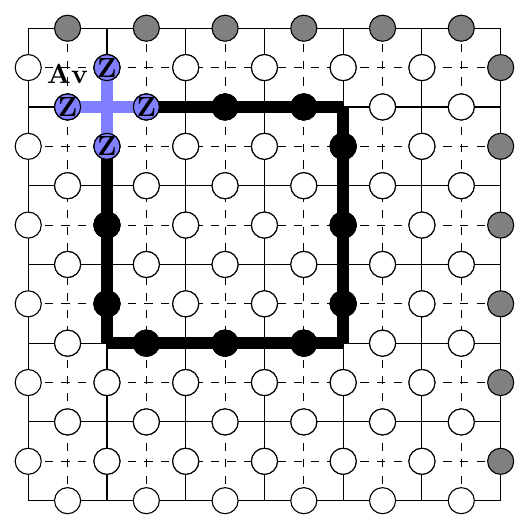
\begin{tikzpicture}
	% Draw dashed lines
	\foreach \i in {-3,-2.5,...,3}
	{
		\draw[dashed] (\i,-3) -- (\i,3);
	}
	\foreach \j in {-3,-2.5,...,3}
	{
		\draw[dashed] (-3,\j) -- (3,\j);
	}
	
	
	
	% Draw solid grid and nodes with circles in the middle of each side
	\draw[step=1cm] (-3,-3) grid (3,3);
	\foreach \i in {-2.5,...,2.5}
	{
		\foreach \j in {-2.5,...,2.5}
		{
			
			
			\begin{scope}[transform canvas={xshift=\i cm,yshift=\j cm}]
				\node[right,xshift=0.2cm,yshift=0.4cm] {};
				% Convert \j and \i to integers
				\pgfmathtruncatemacro{\intj}{\j}
				\pgfmathtruncatemacro{\inti}{\i}
				
				% Draw circles at the midpoints of each side
				\ifnum\intj=2
				\draw node[draw,circle,fill=gray] at (0,0.5) {};
				\else
				\draw node[draw,circle,fill=white] at (0,0.5) {};
				\fi
				
				\ifnum\inti=2
				\draw node[draw,circle,fill=gray] at (0.5,0) {};
				\else
				\draw node[draw,circle,fill=white] at (0.5,0) {};
				\fi
				
				\draw node[draw,circle,fill=white] at (0,-0.5) {};
				\draw node[draw,circle,fill=white] at (-0.5,0) {};
			\end{scope}
		}
	}
	
	\foreach \i in {-2,...,-2}
	{
		\draw[black, line width=1.5mm] (\i,-1) -- (\i,1.5);
		\node[draw, circle, fill=black] at (\i,-0.5) {};
		\node[draw, circle, fill=black] at (\i,0.5) {};
		
		\draw[blue!50, line width=1.5mm] (\i,1.5) -- (\i,2.5);
		\node[draw, circle, fill=blue!50,label=center:\textbf{Z}] at (\i,1.5) {};
		\node[draw, circle, fill=blue!50,label=center:\textbf{Z}] at (\i,2.5) {};
		
		
	}
	
	\foreach \j in {2,...,2}
	{
		
		\draw[blue!50, line width=1.5mm] (-2.5, \j) -- (-1.5, \j);
		
		
		\draw[black, line width=1.5mm] (-1.5, \j) -- (1, \j);
		\draw node[draw,circle,fill=black] at (-0.5,\j) {};
		\draw node[draw,circle,fill=black] at (0.5,\j) {};
		\draw node[draw,circle,fill=blue!50,label=center:\textbf{Z},label=north:\textbf{Av}] at (-2.5,\j) {};
		\draw node[draw,circle,fill=blue!50,label=center:\textbf{Z}] at (-1.5,\j) {};
		
	}
	
	
	\foreach \i in {1,...,1}
	{
		\draw[black, line width=1.5mm] (\i,-1) -- (\i,2);
		\node[draw, circle, fill=black] at (\i,-0.5) {};
		\node[draw, circle, fill=black] at (\i,0.5) {};
		\draw node[draw,circle,fill=black] at (\i,1.5) {};
		
	}
	
	\foreach \j in {-1,...,-1}
	{
		\draw[black, line width=1.5mm] (-2, \j) -- (1, \j);
		\draw node[draw,circle,fill=black] at (0.5,\j) {};
		\draw node[draw,circle,fill=black] at (-0.5,\j) {};
		\draw node[draw,circle,fill=black] at (-1.5,\j) {};
	}
	
	
\end{tikzpicture}
\end{center}

\caption{--}
\label{fig:Aveigen}
\end{figure}

